\documentclass[]{article}
\usepackage{amsmath}
%\usepackage{mhchem}
\usepackage{amssymb}
\usepackage{amsthm}
\usepackage{mathtools}
\usepackage{relsize}
\usepackage{algpseudocode}
\usepackage{tikz}

%\usepackage{mathptmx,courier}
\usepackage[scaled=0.92]{helvet}
\normalfont
\usepackage{pifont,tabularx,varioref,url}
\usepackage[T1]{fontenc}
\DeclareMathOperator{\adj}{adj}
\DeclareMathOperator{\A}{\emph{\textbf{A}}}
\DeclareMathOperator{\B}{\emph{\textbf{B}}}

\newcommand{\Z}{\mathbb{Z}}
\newcommand{\R}{\mathbb{R}}
\newcommand{\Q}{\mathbb{Q}}
\newcommand{\N}{\mathbb{N}}

\input{structure.tex} % Include the file specifying the document structure and custom commands

%----------------------------------------------------------------------------------------
%	ASSIGNMENT INFORMATION
%----------------------------------------------------------------------------------------

% Required
\newcommand{\assignmentQuestionName}{P} % The word to be used as a prefix to question numbers; example alternatives: Problem, Exercise
%\newcommand{\assignmentClass}{} % Course/class
\newcommand{\assignmentTitle}{\text{CS201 Assignment 2}} % Assignment title or name
\newcommand{\assignmentAuthorName}{Pathe Nevish Ashok (220757)}

% Optional (comment lines to remove)
%\newcommand{\assignmentClassInstructor}{ } % Intructor name/time/description
%\newcommand{\assignmentDueDate}{ } % Due date

\begin{document}
	\begin{center}
		{\LARGE CS201 Assignment 2: The Concept of Graphs}
	\end{center}
	
	\vspace{3mm}
	{\large \hfill Maximum Marks: $100$}
	
	\vspace{10mm}
	
	\stuf{Q1.\\Consider the following directed graph; $(1,2),(3,2),(1,4),(3,4)$. We can observe that there does not exist any path between vertices $1$ and $3$ unless we ignore the directions of edges. \\

\begin{center}
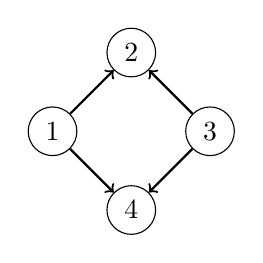
\begin{tikzpicture}
	
	% Nodes
	\node[circle, draw] (1) at (-1,0) {1};
	\node[circle, draw] (3) at (1,0) {3};
	\node[circle, draw] (2) at (0,1) {2};
	\node[circle, draw] (4) at (0,-1) {4};
	
	% Directed edges
	\draw[thick, ->] (1) to (2);
	\draw[thick, ->] (1) to (4);
	\draw[thick, ->] (3) to (2);
	\draw[thick, ->] (3) to (4);
\end{tikzpicture}
\end{center}
	
	}
	
	\stuf{
		Q2.\\ Let us denote the path from a vertex $u$ to another vertex $v$ as $\{u,v\}$. Thus, we show the following properties:\\ \\ \textit{Reflexivity}: The trivial path $\{u,u\}$ having no edges, exists for any vertex $u \implies uRu$.\\
		\textit{Symmetry}: If $uRv$ then $\{u,v\}$ exists as well as $\{v,u\} \implies vRu$.\\
		\textit{Transitivity}: If $uRv$ and $vRw$, then the paths $\{u,v\}, \{v, w\}$ as well as $\{w,v\}, \{v,u\}$ exist, thus, $\{u,w\} = \{u,v\} \cup \{v,w\}$ and $\{w,u\} = \{w, v\} \cup \{v, u\}$ exist $\implies uRw$. 
	}
	
	\stuf{Q3. \\
		Let us assume that all the edges from $V_1$ to $V_2$ are not in the same direction $\implies$ there exists edges $(u,v)$ and $(x,w)$ such that $u, v \in V_1; w,x \in V_2$. Now the paths $\{u,w\},\{w,u\}$ as well as $\{v,x\}, \{x,v\}$ exist (since they are in the same equivalence class). We can have a path from $u\to x$ viz. $\{u,v\} \cup \{v,x\}$, and likewise for $x \to u : \{x,w\} \cup \{w,u\}$. But this means that $u$ and $x$ belong to the same equivalence class, which is a contradiction. 
	}
	
	\stuf{Q4. \\
		Let us prove $|E| = |V| - 1$ by induction on the number of vertices. The case of one node is trivial with $0$ edges. Assuming it holds for $(n-1)$ vertices, Consider a directed tree with $n$ vertices. We can always choose a leaf vertex (vertex with $\mathbf{inDegree} = 1$ and $\mathbf{outDegree} = 0$). Thus, we can remove it and the incoming edge out of the graph and obtain a tree with $(n-1)$ edges satisfying the equation. Thus, on adding it back again, number of edges as well as vertices go up by exactly one. Thus, $|E| + 1 = |V| + 1 - 1$ i.e. $|E'| = |V'| - 1$ is still satisfied.\\
		
		On neglecting the direction of edges, we should have a connected graph with $n$ vertices and $(n-1)$ edges i.e. a tree and a cycle cannot exist. Thus, we cannot have path from $v$ to $u$, if a path from $u$ to $v$ exists (otherwise, it'd contradict the connectivity of the tree/graph).
		
	}
	
	\stuf{Q5. \\
		For any set of $n$ vertices, WLOG, we can label the vertices from $1$ to $n$. Now, for each $i \in \{1, 2, ..., n\}$, we can divide it into sets with numbers smaller and that of larger than $i$ viz. $\{..., i-1\}, \{i+1, ...\}$ having $(i-1)$ and $(n-i)$ elements respectively. Now, to form a binary search tree, we can construct it by taking $i$ as a root and partitioning rest of the nodes as above. Thus, we can recursively write $T_n$ as the sum of all possible BSTs over all roots $i$ i.e. summing over the terms $T_{i-1} T_{n-i}$. \\
		This is because since we want to find the number of drawings, the $(i-1)$ and $(n-i)$ can be \textit{any} vertices, so we chose the above configuration.\\
		The base cases $T_0 = 1, T_1 = 1$ respectively for an empty BST and a BST with single node. $T_n = \sum\limits_{i=1}^{n} T_{i-1} T_{n-i}$. Thus, this gives us the total number of drawings of binary trees possible. 
	}
	
	\stuf{Q6. \\
		For unlabelled binary trees (i.e. the number of drawings), we use the above recurrence relation. Consider the generating function $G(x) = \sum\limits_{n\ge0} T_n x^n$. Thus,\\
		
		\begin{align*}
			\displaystyle G(x) &= \sum\limits_{n\ge0} T_n x^n \\
			&= \sum\limits_{n\ge 0} \sum\limits_{i=1}^{n} T_{i-1} T_{n-i} x^n = \sum\limits_{n\ge 0} \sum\limits_{i=0}^{n-1} T_{i} T_{n-i-1} x^n \\
			&= 1 + \sum\limits_{n\ge 1} \sum\limits_{i=0}^{n-1} T_{i} T_{n-i-1} x^n\\
			(t:&=n-1)\\
			&= 1 + x\left(\sum\limits_{t\ge 0} \sum\limits_{i=0}^{t} T_{i} T_{t-i} x^t \right)\\
			&\text{By convolution of generating functions,}
			\\
			&= 1 + x \left(\sum\limits_{t\ge 0} T_t x^t \right) \left(\sum\limits_{t\ge 0} T_t x^t \right)\\
			&= 1 + x \left( \sum\limits_{t\ge 0} T_t x^t \right)^2\\
			&= 1 + x G(x)^2\\
			\implies G(x) &= \frac{1\pm \sqrt{1-4x}}{2x}
		\end{align*}
		Taking the negative square root since,
		$G(0) = \lim_{x\to0} \frac{1-\sqrt{1-4x}}{2x} = \lim_{x\to 0} \frac{2}{1+\sqrt{1+4x}} = 1 = T_0$ (doesn't work for the positive root)\\
		
		\begin{align*}
			\textrm{as discussed in the class...}\\
			\left(1-4x\right)^{1/2}&=1+\sum_{n\ge 1}\binom{1/2}n(-4x)^n\\
			&=1+\sum_{n\ge 1}\frac{\left(\frac12\right)\left(-\frac12\right)\left(-\frac32\right)\dots\left(-\frac{2n-3}2\right)}{n!}(-4x)^n\\
			&=1+\sum_{n\ge 1}(-1)^{n-1}\frac{(2n-3)!!}{2^nn!}(-4x)^n\\
			&=1-\sum_{n\ge 1}\frac{2^n(2n-3)!!}{n!}x^n\\
			&=1-2\sum_{n\ge 1}\frac{2^{n-1}\prod_{k=1}^{n-1}(2k-1)}{n(n-1)!}x^n\\
			&=1-2\sum_{n\ge 1}\frac{2^{n-1}(n-1)!\prod_{k=1}^{n-1}(2k-1)}{n(n-1)!^2}x^n\\
			&=1-2\sum_{n\ge 1}\frac{\left(\prod_{k=1}^{n-1}(2k)\right)\left(\prod_{k=1}^{n-1}(2k-1)\right)}{n(n-1)!^2}x^n\\
			&=1-2\sum_{n\ge 1}\frac{(2n-2)!}{n(n-1)!^2}x^n\\
			&=1-2\sum_{n\ge 1}\frac1n\binom{2(n-1)}{n-1}x^n\;,
		\end{align*}
		
		\begin{align*}
			G(x)&=\frac1{2x}\cdot2\sum_{n\ge 1}\frac1{n}\binom{2(n-1)}{n-1}x^n\\
			&=\sum_{n\ge 1}\frac1n\binom{2(n-1)}{n-1}x^{n-1}\\
			&=\sum_{n\ge 0}\frac1{n+1}\binom{2n}nx^n\;,
		\end{align*}
		
		\begin{align*}
			\implies \boxed{T_n = \frac{1}{n+1} \binom{2n}{n}}
		\end{align*}
	}
	
	\stuf{Q7. \\
		Consider that edges are directed from $V_1 \to V_2$, $V_2 \to V_3$ and $V_1 \to V_3$. Thus, $H$ contains the edges $(1,2), (2,3)$ and $(1,3)$ with $\mathbf{inDegree}(3) = 2$. Thus, $H$ may not always be a tree. 
		
		\begin{center}
			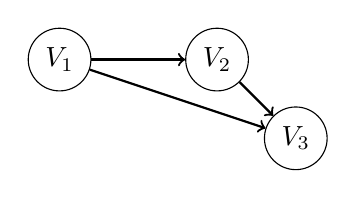
\begin{tikzpicture}
				
				% Nodes
				\node[circle, draw] (1) at (-1,0) {$V_1$};
				\node[circle, draw] (2) at (1,0) {$V_2$};
				\node[circle, draw] (3) at (2,-1) {$V_3$};

				
				% Directed edges
				\draw[thick, ->] (1) to (2);
				\draw[thick, ->] (1) to (3);
				\draw[thick, ->] (2) to (3);
			\end{tikzpicture}
		\end{center}
	}
	
	\stuf{Q8. \\
		We have defined a tree as an undirected graph having a unique path between any two vertices. 
		$(\implies)$\\
		Assuming the graph is connected and does not have any cycles. Suppose there are multiple paths between two vertices $u$ and $w$. Consider any two of them, $\{u, v_1, v_2, v_3, ..., w\}$ and $\{u, x_1, x_2, .., w\}$. We have a cycle $\{u, v_1, v_2, ..., w, ..., x_2, x_1, u\}$. Thus, there cannot exist more than one path and since the graph is connected we have a unique path between each pair of vertices. \\
		$(\impliedby)$\\
		Since there exists a unique path between any pair of vertices, the graph is connected. Now, if a cycle $\{u, ..., v, ..., u\}$ were to exist with vertices $u$ and $v$ lying on it, we'd have two distinct paths from $u$ to $v$, $\{u, ..., v\}$ and $\{v, ..., u\}$, hence a contradiction. So, a cycle cannot exist.
		\qed
	}
	
	\stuf{Q9. \\
		Similar to Q3, we assume two strongly connected graphs $V_1, V_2$ having the vertices $v_1, v_2$ respectively. Now, if a cycle exists with $v_1, v_2$ lying on it, any vertex in $V_2$ can be reached from a vertex in $V_1$ by following the directed part $v_1 \to v_2$ of the cycle and then further from $v_2$ to that vertex in $V_2$. Likewise, any vertex in $V_1$ can be reached from that in $V_2$ and thus all the vertices belong to the same connected component, a contradiction. Hence, a cycle in a directed graph has all its vertices belonging to the same connected component.   
	}
	
	\stuf{Q10. \\
		$(\implies)$\\
		If an undirected graph is connected, then there is at least one path between any two vertices and multiple paths imply cycles. Thus, we can remove edges from cycles and until it doesn't affect the connectivity of the graph. At this point, we have a unique path between any two vertices and thus, a spanning tree is obtained. If we cannot delete such edges, then the original graph itself is a tree and thus a spanning tree too.\\
		$(\impliedby)$\\
		Since a spanning tree is a subgraph of the original graph, connectedness of spanning tree implies connectedness of the original graph.
	}
	
	\stuf{Q11. \\
		(Assuming that we are considering a \textit{connected} minimum weight subgraph)\\
		If all the weights are positive, then the minimum weight subgraph would be the minimum spanning tree itself because the minimum weight connected subgraph must be a tree; If it contains a cycle, then we can remove the edge with largest weight and still ensure connectivity. Thus, it is a spanning tree and has minimum weight giving us an MST.\\
		
		While, if the graph has negative weights as well, then the minimum weight subgraph (may or may not be connected) need not be a spanning tree since it may contain cycles, and if we remove negative-weighted edges to form a spanning tree (possibly), it is no longer the minimum weight subgraph.
	}
	
	\stuf{Q12. \\
		Let the minimum spanning tree of given graph $G(V,E,w)$ be $M$. Let $T$ denote the graph formed by the algorithm in the intermediate steps. At the first step $T$ is a trivial subgraph of $M$ with a single vertex $v$. Now, we claim that at the end of each iteration $2-3-4-5-2$,  $T$ is a subgraph of MST $M$. We invoke induction on the number of iterations.\\
		
		Thus, let the above be true after some $k$ iterations. In the next one, we add some edge $e_{ij} = (v_i, v_j)$ according to the algorithm. Now, if $e_{ij} \in M$, $T \cup e_{ij}$  is a subgraph of $M$ and we are done.\\
		If $e_{ij}$ isn't in $M$, then we add it. But this gives us a cycle since $M$ is an MST (minimally acyclic). Since $v_i \in T, v_j \not\in T$, there must exist some edge $e_{pq}\in M$ where $v_p \in T, v_q \not\in T$ (otherwise a cycle won't exist). According to the algorithm, $w(e_{ij}) \le w(e_{pq})$ (comparing weights). We can remove $e_{pq}$ from $M$, giving us an MST such that the assumption $T \cup e_{ij}$ being a subgraph of $M$ holds. This is the inductive step.\\
		
		After $(n-1)$ iterations, the same number of edges are added i.e. we have $T$ with $n$ vertices and $(n-1)$ edges, just like the MST $M$. Thus $T = M$ since it is a subgraph of $M$.
	}
	
	\stuf{Q13. \\
		(Assuming positive weights)\\
		Consider a minimum length tour $T$ and an MST $M$ of the given graph. Since $T$ starts and ends on the same vertex, while traversing each edge atmost once, we can remove an edge and still ensure connectivity. It would give us a spanning tree $T'$. The inequality on total weights $w(M) \le w(T') \le w(T)$ follows.
	}
	
	\stuf{Q14. \\
		Consider the minimum spanning tree $M$ of the given graph and the minimum length tour $T^*$. Performing a DFS traversal of $M$ gives a tour $T$ which traverses each edge exactly twice, thus giving the total weight of the tour, $w(T) = 2w(M)$.  This is indeed an Eulerian Circuit on the resultant Eulerian (multi)Graph formed by doubling each edge in the $MST$ (exists since all vertices have even degree, as discussed in the class). Thus, we have $w(M) \le w(T^*)$ and $w(M) \le w(T) = 2w(M)$.\\
		
		If it is possible, in some way, to reduce this tour such that we reach the minimum length tour, we are done. The Eulerian circuit above visits each vertex multiple times. Thus, say, we have the vertices $v_1, v_2, v_3$ and the circuit follows $\to v_1 \to v_2 \to v_3 \to$ and also $\gets v_1 \gets v_2 \gets v_3 \gets$. If we could skip $v_2$ the second time, it'd give us a tour with smaller weight.  Thus, a crucial assumption; $w(v_1, v_2) + w(v_2, v_3) \ge w(v_1,v_3)$ for all such $v_1, v_2, v_3$ helps us to reduce the tour. Thus, the optimal tour $T^*$ follows the inequality, $w(M) \le w(T^*) \le w(T) = 2w(M)$.
		
		For example, the graph in {\color{red}{red}} is the MST of below graph and black-{\color{blue}{blue}} edges show the DFS tour.
		\begin{center}
		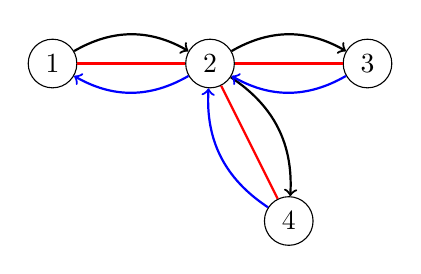
\begin{tikzpicture}
			% Nodes
			\node[circle, draw] (1) at (0,0) {1};
			\node[circle, draw] (2) at (2,0) {2};
			\node[circle, draw] (3) at (4,0) {3};
			\node[circle, draw] (4) at (3,-2) {4};
			

			% Tour with double edges
			\draw[thick,->,bend left] (1) to (2);
			\draw[thick,->,bend left] (2) to (3);
			\draw[thick,->,bend left] (2) to (4);

			
			% Double edges
			\draw[thick,->,bend left, color = blue] (2) to (1);
			\draw[thick,->,bend left, color = blue] (3) to (2);
			\draw[thick,->,bend left, color = blue] (4) to (2);
			
			 \draw[thick, color=red] (1) -- (2);
			\draw[thick, color=red] (2) -- (3);
			\draw[thick, color=red] (2) -- (4);
			

		\end{tikzpicture}
		\end{center}
	}
	
\end{document}